\documentclass{article}
\usepackage[utf8]{inputenc}
\usepackage{amsmath}
\usepackage{bm}
\usepackage[a4paper, inner=2.5cm, outer=2.5cm, top=2.5cm, bottom=2.5cm]{geometry}
\usepackage{graphicx}
\graphicspath{{figures/}}

\title{Classical Laminate Theory}
\author{Andy Perez}
\date{February 2019}

\begin{document}
\setlength{\parindent}{0cm}
\renewcommand{\thefootnote}{\roman{footnote}}

\maketitle

This document provides a summarized walk-through of Classical Laminate Theory (CLT) using NASA Reference Publication 1351 \textit{Basic Mechanics of Laminate Composite Plates} \cite{nasa} as a reference. Supplemental and original source information is also found in Jones' \textit{Mechanics of Composite Materials} \cite{jones}


\section{Lamina Properties}
\label{sec:lamina_properties}
Basic material properties are determined empirically, and must be known in order to determine the lamnia's characteristic matrices and the resulting loads and stresses. These values are:
  \begin{center}
    \begin{table}[h!]
      \centering
      \label{tbl:lamprop}
      \vspace{1mm}
      \begin{tabular}{cl}
        Symbol & Description \\
        \hline \hline
        $\bm{E_{11}}$ & elastic modulus in the ply's 0$^{\circ}$-direction \\
        $\bm{E_{22}}$ & elastic modulus in the ply's 90$^{\circ}$-direction \\
        $\bm{\nu_{12}}$ & Poisson's ratio in the $2$-direction when the lamina is loaded in the $1$-direction \\
        $\bm{G_{12}}$ & Shear modulus in the $12$-plane \\
        $\bm{t_{k}}$ & thickness of the lamina \\
        $\bm{\alpha_{11}}$ & thermal expansion coefficient in the in the ply's 0$^{\circ}$-direction \\
        $\bm{\alpha_{12}}$ & thermal expansion coefficient in the in the ply's 90$^{\circ}$-direction \\
        $\bm{\beta_{11}}$ & hygral expansion coefficient in the in the ply's 0$^{\circ}$-direction \\
        $\bm{\beta_{12}}$ & hygral expansion coefficient in the in the ply's 90$^{\circ}$-direction \\
        $\bm{\theta}$ & the ply orientation (used for off-axis transformations)
      \end{tabular}
    \end{table}
  \end{center}


\section{Characteristic Matrices of the Lamina}
\label{sec:lamina_matrices}
Note that, in general, the subscript $k$ is used to denote that the a value is a lamina value. The characteristic matrices for each lamina can be calculated as follows:

  \begin{enumerate}
    \item The \emph{reduced stiffness matrix} $\bm{Q_{k}}$ describes the elastic behavior of the ply in in-plane loading.\footnote{$Q_{k}$ is derived from Staab \cite{staab}, Eq. 3.9, while the values for $Q_{11}$, $Q_{22}$, and $Q_{12}$ are from Nettles \cite{nasa}, Eq. (10).}
      \begin{equation}
        \label{var:Qk} % Staab Eq. 3.9
        \bm{Q_{k}} = \left[
                        \begin{array}{ccc}
                          Q_{11} & Q_{12} & 0 \\
                          Q_{12} & Q_{22} & 0 \\
                          0  &      0     & Q_{66}
                        \end{array}
                      \right]
      \end{equation}
      where
      $$
        Q_{11} = \frac{E_{11}^{2}}{\left(E_{11} - \nu_{12} \cdot E_{22}\right)}
      $$ \vspace{1mm}
      $$
        Q_{22} = \frac{E_{11} E_{22}}{\left(E_{11} - \nu_{12}^2 E_{22}\right)}
      $$ \vspace{1mm}
      $$
      Q_{12} = \frac{\nu_{12} E_{11} E_{22}}{\left(E_{11} - \nu_{12}^2 E_{22}\right)}
      $$ \vspace{1mm}
      $$
        Q_{66} = G_{12}
      $$
    \item The \emph{strain transformation matrix} $\bm{T_{\varepsilon}}$ is used to transform other characteristic matrices into the laminate coordinate system.\footnote{Staab \cite{staab}, Eq 2.1}
    \begin{equation}
      \label{var:Tepsilon} % Staab Eq. 2.1
      \bm{T_{\varepsilon}} = \left[ \begin{array}{ccc}
                                      m^{2} & n^{2} & mn \\
                                      n^{2} & m^{2} & -mn \\
                                      -2mn & 2mn & m^{2} - n^{2} \\
                                    \end{array}
                             \right]
    \end{equation}
    where
    $$m=\cos\theta$$
    $$n=\sin\theta$$
    $\theta$ is the relative orientation of the lamina with respect to the laminate coordinate system shown in Figure~\ref{fig:ply_axes}\footnote{\emph{ibid.}, Fig. 3.3}.
    \begin{figure}[h] % Staab Figure 3.3
      \centering
      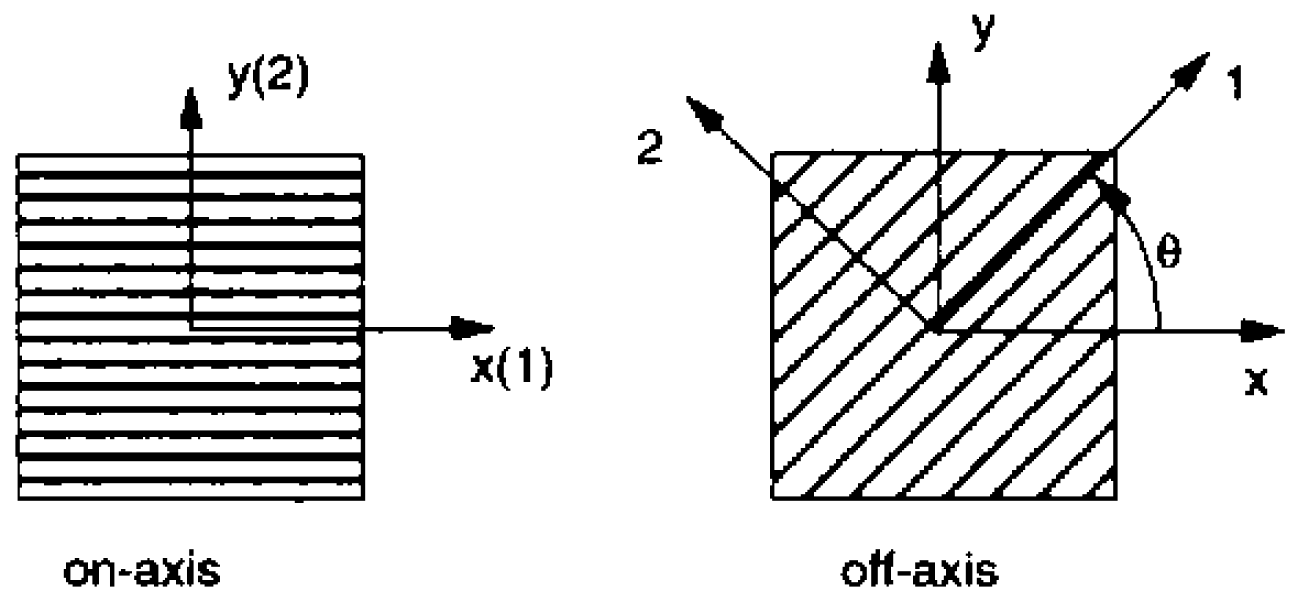
\includegraphics[scale=.25]{staab_fig_3-3.png}
      \caption{On- and Off-axis Ply Orientations}
      \label{fig:ply_axes}
    \end{figure}

  \item The \emph{stress transformation matrix} $\bm{T_{\sigma}}$, by comparison, is calculated by the following equation.\footnote{\emph{ibid.}, Eq. 2.3}
    \begin{equation}
      \label{var:Tsigma}
      \bm{T_{\sigma}} = \left[
                          \begin{array}{ccc}
                            m^{2} & n^{2} & 2mn \\
                            n^{2} & m^{2} & -2mn \\
                            -mn & mn & m^{2} - n^{2} \\
                          \end{array}
                        \right]
    \end{equation}
    It should be noted that if tensor notation is used for both strains, then the stress and strain transformation matrices should be equal, $\bm{T_{\varepsilon}} = \bm{T_{\sigma}}$.

  \item The \emph{transformed reduced stiffness matrix} $\bm{\overline{Q}_{k}}$ is calculated by modifying $Q_{k}$ by $T_{\varepsilon}$ \footnote{\emph{ibid.} Section 3.2.2}.
    \begin{equation}
      \label{var:Qbar}
      \bm{\overline{Q}_{k}} = \bm{T_{\sigma}}^{-1} \bm{Q_{k}} \bm{T_{\varepsilon}}
    \end{equation}

  \end{enumerate}

\section{Determining the $\bm{A}$, $\bm{B}$, and $\bm{D}$ Matrices}
When lamina are bonded together to form a laminate, there exist three matrices that characterize the stiffness of the laminate. These are the \emph{extensional stiffness matrix} $\bm{A}$, the \emph{extension-bending stiffness matrix} $\bm{B}$, and the \emph{bending stiffness matrix} $\bm{D}$.
  \subsection{The Extensional Stiffness Matrix}
  The \emph{extensional stiffness matrix} $\bm{A}$ characterizes the axial, in-plane stiffness of the laminate and is defined
  \begin{equation}
    \bm{A} = \left[ \begin{array}{ccc}
               A_{11} & A_{12} & A_{16} \\
               A_{12} & A_{22} & A_{26} \\
               A_{16} & A_{26} & A_{16} \\
             \end{array} \right]
  \end{equation}
  where
  \begin{equation}
    A_{ij} = \sum_{k=1}^{n}\big[\overline{Q}_{ij}\big]_{k}\big(z_{k} - z_{k-1}\big)
  \end{equation}

  \subsection{The Extension-Bending Coupling Matrix}
  The \emph{extension-bending coupling matrix} $\bm{B}$ couples the extensional stiffness and the bending stiffness matrices. It is defined:
  \begin{equation}
    \bm{B} = \left[ \begin{array}{ccc}
               B_{11} & B_{12} & B_{16} \\
               B_{12} & B_{22} & B_{26} \\
               B_{16} & B_{26} & B_{16} \\
             \end{array} \right]
  \end{equation}
  where
  \begin{equation}
    B_{ij} = \frac{1}{2}\sum_{k=1}^{n}\big[\overline{Q}_{ij}\big]_{k}\big(z_{k}^{2} - z_{k-1}^{2}\big)
  \end{equation}

  \subsection{The Bending Stiffness Matrix}
  The \emph{bending stiffness matrix} $\bm{B}$ characterizes the stiffness of the laminate when subjected to bending loads and is defined:
  \begin{equation}
    \bm{D} = \left[ \begin{array}{ccc}
               D_{11} & D_{12} & D_{16} \\
               D_{12} & D_{22} & D_{26} \\
               D_{16} & D_{26} & D_{16} \\
             \end{array} \right]
  \end{equation}
  where
  \begin{equation}
    D_{ij} = \frac{1}{3}\sum_{k=1}^{n}\big[\overline{Q}_{ij}\big]_{k}\big(z_{k}^{3} - z_{k-1}^{3}\big)
  \end{equation}

  \subsection{The $\bm{ABD}$ Matrix}
  Together, all three stiffness matrices fully characterize the laminate stiffness and can be used to relate applied loads to the resulting strains on a laminate and in its lamina. This relationship is defined as
    \begin{equation}
      \left\{\begin{array}{c} \bm{N} \\ \hline \bm{M} \end{array} \right\} = \left[\begin{array}{c|c} \bm{A} & \bm{B} \\ \hline \bm{B} & \bm{D} \end{array} \right] \left\{ \begin{array}{c} \bm{\varepsilon^{0}} \\ \hline \bm{\kappa} \end{array} \right\}
    \end{equation}
  which, when expanded, becomes
  \begin{equation}
      \left\{\begin{array}{c} N_{xx}'\\
                             N_{yy}'\\
                             N_{xy}'\\
                             \hline
                             M_{xx}'\\
                             M_{yy}'\\
                             M_{xy}'\\
      \end{array} \right\} =
      \left[ \begin{array}{ccc|ccc} A_{11} & A_{12} & A_{16} & B_{11} & B_{12} & B_{16} \\
                                  A_{21} & A_{22} & A_{26} & B_{21} & B_{22} & B_{26} \\
                                  A_{61} & A_{62} & A_{66} & B_{61} & B_{62} & B_{66} \\
                                  \hline
                                  B_{11} & B_{12} & B_{16} & D_{11} & D_{12} & D_{16} \\
                                  B_{21} & B_{22} & B_{26} & D_{21} & D_{22} & D_{26} \\
                                  B_{61} & B_{62} & B_{66} & D_{61} & D_{62} & D_{66} \\
              \end{array} \right]
      \left\{ \begin{array}{c} \varepsilon_{xx}^{0} \\ \varepsilon_{yy}^{0} \\ \gamma_{xy}^{0} \\ \hline \kappa_{xx} \\ \kappa_{yy} \\ \kappa_{xy} \end{array}\right\}
  \end{equation}

\bibliographystyle{ieeetr}
\bibliography{clt}


\section{Creating the ABD Matrix}
The ABD matrix is a 6x6 matrix that serves as a connection between the applied loads and the associated strains in the laminate. It essentially defines the elastic properties of the entire laminate. To assemble the ABD matrix, follow these steps:

\begin{enumerate}
    \item Calculate reduced stiffness matrix $\bm{Q_{k}}$ for each material used in the laminate (if a laminate uses only one type of composite material, there will be only 1 stiffness matrix). The stiffness matrix describes the elastic behavior of the ply in plane loading

    \begin{equation}
        \bm{Q_{k}} = \left[ \begin{array}{ccc}
                                Q_{11} & Q_{12} & 0 \\
                                Q_{21} & Q_{22} & 0 \\
                                0  &      0     & Q_{66}
                            \end{array} \right]
    \end{equation}
    where

    $$
        Q_{11} = \frac{E_{11}^{2}}{\left(E_{11} - \nu_{12} \cdot E_{22}\right)}
    $$ \vspace{1mm}
    $$
        Q_{12} = \frac{\nu_{12} E_{11} E_{22}}{\left(E_{11} - \nu_{12}^2 E_{22}\right)}
    $$ \vspace{1mm}
    $$
        Q_{22} = \frac{E_{11} E_{22}}{\left(E_{11} - \nu_{12}^2 E_{22}\right)}
    $$ \vspace{1mm}
    $$
        Q_{66} = G_{12}
    $$

    where

    $$
        Q_{11} = \frac{E_{11}^{2}}{\left(E_{11} - \nu_{12} \cdot E_{22}\right)}
    $$ \vspace{1mm}
    $$
        Q_{12} = \frac{\nu_{12} E_{11} E_{22}}{\left(E_{11} - \nu_{12}^2 E_{22}\right)}
    $$ \vspace{1mm}
    $$
        Q_{22} = \frac{E_{11} E_{22}}{\left(E_{11} - \nu_{12}^2 E_{22}\right)}
    $$ \vspace{1mm}
    $$
        Q_{66} = G_{12}
    $$

    \item Calculate the transformed reduced stiffness matrix $\bm{\overline{Q_{k}}}$ for each ply based on the reduced stiffness matrix and fiber angle.
    \begin{equation}
        \bm{\overline{Q}_{k}} =
        \left[ \begin{array}{ccc}
            \overline{Q}_{11} & \overline{Q}_{12} & \overline{Q}_{16} \\
            \overline{Q}_{21} & \overline{Q}_{22} & \overline{Q}_{26} \\
            \overline{Q}_{61} & \overline{Q}_{62} & \overline{Q}_{66}
        \end{array} \right]
    \end{equation}

    where \\
    $$
        \overline{Q}_{11} = Q_{11}\cos^{4}(\theta) + 2\big(Q_{12} + Q_{66}\big)\cos^{2}(\theta)\cdot\sin^{2}(\theta) + Q_{22}\sin^{4}(\theta)
    $$
    $$
        \overline{Q}_{12} = \overline{Q}_{21} = Q_{12}\big(\cos^{4}(\theta) + \sin^{4}(\theta)\big) + \big(Q_{11} + Q_{22} - 4Q_{66}\big)\cos^{2}(\theta)\sin^{2}(\theta)
    $$
    $$
        \overline{Q}_{16} = \overline{Q}_{61} = \big(Q_{11} - Q_{12} - 2Q_{66}\big)\cos^{3}(\theta)\sin(\theta) - \big(Q_{22} - Q_{12} - 2Q_{66}\big)\cos(\theta)\sin^{3}(\theta)
    $$
    $$
        \overline{Q}_{22} = Q_{11}\sin^{4}(\theta) + 2\big(Q_{12} + Q_{66}\big)\cos^{2}(\theta)\cdot\sin^{2}(\theta) + Q_{22}\cos^{4}(\theta)
    $$
    $$
        \overline{Q}_{26} = \overline{Q}_{62} = \big(Q_{11} - Q_{12} - 2Q_{66}\big)\cos(\theta)\sin^{3}(\theta) - \big(Q_{22} - Q_{12} - 2Q_{66}\big)\cos^{3}(\theta)\sin(\theta)
    $$
    $$
        \overline{Q}_{66} = \big(Q_{11} + Q_{22} - 2Q_{12} - 2Q_{66}\big)\cos^{2}(\theta)\sin^{2}(\theta) + Q_{66}\big(\cos^{4}(\theta) + \sin^{4}(\theta)\big)
    $$

    \item Calculate the laminate \emph{extensional stiffness matrix}, $\bm{A}$:
    \begin{equation}
    \bm{A} = \left[\begin{array}{ccc} A_{11} & A_{12} & A_{16} \\ A_{21} & A_{22} & A_{26} \\ A_{61} & A_{62} & A_{66}\end{array}\right]
    \end{equation}
    The individual terms of $\bm{A}$ are calculated by
    \begin{equation}
        A_{ij} = \sum_{k=1}^{n} \big\{Q_{ij}\big\}_{n} \left(z_{k} - z_{k-1}\right)
    \end{equation}
    where $z$ is the vertical position in the ply from the midplane, and $k$ is for each ply.

    \item Calculate the laminate \emph{coupling stiffness matrix}, $\bm{B}$:
    \begin{equation}
        \left[\begin{array}{ccc} B_{11} & B_{12} & B_{16} \\ B_{21} & B_{22} & B_{26} \\ B_{61} & B_{62} & B_{66}\end{array}\right]
    \end{equation}
    where
    \begin{equation}
        B_{ij} = \frac{1}{2} \sum_{k=1}^{n} \big\{Q_{ij}\big\}_{n} \left(z_{k}^{2} - z_{k-1}^{2}\right)
    \end{equation}

    \item Calculate the laminate \emph{bending stiffness matrix}, $\bm{D_{ij}}$:
    \begin{equation}
        \left[\begin{array}{ccc} D_{11} & D_{12} & D_{16} \\ D_{21} & D_{22} & D_{26} \\ D_{61} & D_{62} & D_{66}\end{array}\right]
    \end{equation}
    where
    \begin{equation}
        D_{ij} = \frac{1}{3} \sum_{k=1}^{n} \big\{Q_{ij}\big\}_{n} \left(z_{k}^{3} - z_{k-1}^{3}\right)
    \end{equation}

    \item Assemble the $\bm{ABD}$ matrix:
    \begin{equation}
        \bm{ABD} = \left[\begin{array}{c|c}
            \bm{A} & \bm{B} \\
            \hline
            \bm{B} & \bm{D}
        \end{array} \right]
    \end{equation}
    \end{enumerate}

\section{Laminate Properties}
Overall laminate properties can be calculated from the $\bm{ABD}$ matrix.
\begin{equation}
    \left\{\begin{array}{c} \bm{N} \\ \hline \bm{M} \end{array} \right\} = \left[\begin{array}{c|c} \bm{A} & \bm{B} \\ \hline \bm{B} & \bm{D} \end{array} \right] \left\{ \begin{array}{c} \bm{\varepsilon^{0}} \\ \hline \bm{\kappa} \end{array} \right\}
\end{equation}

\begin{equation}
    \left\{ \begin{array}{c} Q_{x} \\ Q_{y} \end{array} \right\} =
    \left[ \begin{array}{cc} A_{55} & A_{45} \\ A_{45} & A_{44} \end{array} \right]_{k}
    \left\{ \begin{array}{c} \gamma_{xz} \\ \gamma_{yz} \end{array} \right\}_{k}
\end{equation}
where
\begin{equation}
    A_{ij} = c \sum_{k=1}^{N} \left[ \overline{Q}_{ij} \right]_{k} \left\{ \big(z_{k} - z_{k-1} \big) - \frac{4}{3h^{2}} \big(z_{k}^3 - z_{k-1}^3 \big) \right\}
\end{equation}
where $i,j=4,5$ and $c=6/5$ for a rectangular section. Generally speaking, the stiffness terms ($\overline{Q}_{44}$, $\overline{Q}_{55}$, etc.) associated with $Q_{x}$ and $Q_{y}$ are difficult to experimentally determine and are, therefore, approximated.

\begin{equation}
    \left\{\begin{array}{c} N_{xx}'\\
                           N_{yy}'\\
                           N_{xy}'\\
                           \hline
                           M_{xx}'\\
                           M_{yy}'\\
                           M_{xy}'\\
    \end{array} \right\} =
    \left[ \begin{array}{ccc|ccc} A_{11} & A_{12} & A_{16} & B_{11} & B_{12} & B_{16} \\
                                A_{21} & A_{22} & A_{26} & B_{21} & B_{22} & B_{26} \\
                                A_{61} & A_{62} & A_{66} & B_{61} & B_{62} & B_{66} \\
                                \hline
                                B_{11} & B_{12} & B_{16} & D_{11} & D_{12} & D_{16} \\
                                B_{21} & B_{22} & B_{26} & D_{21} & D_{22} & D_{26} \\
                                B_{61} & B_{62} & B_{66} & D_{61} & D_{62} & D_{66} \\
            \end{array} \right]
    \left\{ \begin{array}{c} \varepsilon_{xx}^{0} \\ \varepsilon_{yy}^{0} \\ \gamma_{xy}^{0} \\ \hline \kappa_{xx} \\ \kappa_{yy} \\ \kappa_{xy} \end{array}\right\}
\end{equation}
where $N'$ and $M'$ are the total running loads, including thermal and hygral effects:
\begin{equation}
    N_{ij}' = N_{ij} + N_{ij}^T + N_{ij}^M
\end{equation}
\begin{equation}
    M_{ij}' = M_{ij} + M_{ij}^T + M_{ij}^M
\end{equation}

\section{Calculating Individual Ply Strains and Stresses}
Having calculated the $\bm{ABD}$ matrix for the laminate, it is possible to then calculate individual ply strains and stresses based on the loads and temperature applied to the laminate.
\begin{enumerate}
    \item Calculate the thermal expansion coefficients for each ply:
    \begin{equation}
        \alpha_{xx} = \alpha_{11} \cos^{2}(\theta) + \alpha_{22} \sin^{2}(\theta)
    \end{equation}
    \begin{equation}
        \alpha_{yy} = \alpha_{11} \sin^{2}(\theta) + \alpha_{22} \cos^{2}(\theta)
    \end{equation}
    \begin{equation}
        \alpha_{xy} = 2\cos(\theta)\sin(\theta)\big(\alpha_{11} - \alpha_{22})
    \end{equation}

    \item Calculate the hygral expansion coefficients for each ply:
    \begin{equation}
        \beta_{xx} = \beta_{11} \cos^{2}(\theta) + \beta_{22} \sin^{2}(\theta)
    \end{equation}
    \begin{equation}
        \beta_{yy} = \beta_{11} \sin^{2}(\theta) + \beta_{22} \cos^{2}(\theta)
    \end{equation}
    \begin{equation}
        \beta_{xy} = 2\cos(\theta)\sin(\theta)\big(\beta_{11} - \beta_{22})
    \end{equation}

    \item Calculate the thermal running loads:
    \begin{equation}
        N_{xx}^{T} = \Delta T \sum_{k=1}^{n} \Big\{\big[\overline{Q_{11}}\alpha_{xx} + \overline{Q_{12}}\alpha_{yy} + \overline{Q_{16}}\alpha_{xy}\big]_{k}\big(z_{k} - z_{k-1}\big)\Big\}
    \end{equation}
    \begin{equation}
        N_{yy}^{T} = \Delta T \sum_{k=1}^{n} \Big\{\big[\overline{Q_{12}}\alpha_{xx} + \overline{Q_{22}}\alpha_{yy} + \overline{Q_{26}}\alpha_{xy}\big]_{k}\big(z_{k} - z_{k-1}\big)\Big\}
    \end{equation}
    \begin{equation}
        N_{xy}^{T} = \Delta T \sum_{k=1}^{n} \Big\{\big[\overline{Q_{16}}\alpha_{xx} + \overline{Q_{26}}\alpha_{yy} + \overline{Q_{66}}\alpha_{xy}\big]_{k}\big(z_{k} - z_{k-1}\big)\Big\}
    \end{equation}

    \begin{equation}
        M_{xx}^{T} = \frac{\Delta T}{2} \sum_{k=1}^{n} \Big\{\big[\overline{Q_{11}}\alpha_{xx} + \overline{Q_{12}}\alpha_{yy} + \overline{Q_{16}}\alpha_{xy}\big]_{k}\big(z_{k}^{2} - z_{k-1}^{2}\big)\Big\}
    \end{equation}
    \begin{equation}
        M_{yy}^{T} = \frac{\Delta T}{2} \sum_{k=1}^{n} \Big\{\big[\overline{Q_{12}}\alpha_{xx} + \overline{Q_{22}}\alpha_{yy} + \overline{Q_{26}}\alpha_{xy}\big]_{k}\big(z_{k}^{2} - z_{k-1}^{2}\big)\Big\}
    \end{equation}
    \begin{equation}
        M_{xy}^{T} = \frac{\Delta T}{2} \sum_{k=1}^{n} \Big\{\big[\overline{Q_{16}}\alpha_{xx} + \overline{Q_{26}}\alpha_{yy} + \overline{Q_{66}}\alpha_{xy}\big]_{k}\big(z_{k}^{2} - z_{k-1}^{2}\big)\Big\}
    \end{equation}

    \item Calculate the hygral expansion running loads:
    \begin{equation}
        N_{xx}^{M} = \Delta T \sum_{k=1}^{n} \Big\{\big[\overline{Q_{11}}\beta_{xx} + \overline{Q_{12}}\beta_{yy} + \overline{Q_{16}}\beta_{xy}\big]_{k}\big(z_{k} - z_{k-1}\big)\Big\}
    \end{equation}
    \begin{equation}
        N_{yy}^{M} = \Delta T \sum_{k=1}^{n} \Big\{\big[\overline{Q_{12}}\beta_{xx} + \overline{Q_{22}}\beta_{yy} + \overline{Q_{26}}\beta_{xy}\big]_{k}\big(z_{k} - z_{k-1}\big)\Big\}
    \end{equation}
    \begin{equation}
        N_{xy}^{M} = \Delta T \sum_{k=1}^{n} \Big\{\big[\overline{Q_{16}}\beta_{xx} + \overline{Q_{26}}\beta_{yy} + \overline{Q_{66}}\beta_{xy}\big]_{k}\big(z_{k} - z_{k-1}\big)\Big\}
    \end{equation}

    \begin{equation}
        M_{xx}^{M} = \frac{\Delta T}{2} \sum_{k=1}^{n} \Big\{\big[\overline{Q_{11}}\beta_{xx} + \overline{Q_{12}}\beta_{yy} + \overline{Q_{16}}\beta_{xy}\big]_{k}\big(z_{k}^{2} - z_{k-1}^{2}\big)\Big\}
    \end{equation}
    \begin{equation}
        M_{yy}^{M} = \frac{\Delta T}{2} \sum_{k=1}^{n} \Big\{\big[\overline{Q_{12}}\beta_{xx} + \overline{Q_{22}}\beta_{yy} + \overline{Q_{26}}\beta_{xy}\big]_{k}\big(z_{k}^{2} - z_{k-1}^{2}\big)\Big\}
    \end{equation}
    \begin{equation}
        M_{xy}^{M} = \frac{\Delta T}{2} \sum_{k=1}^{n} \Big\{\big[\overline{Q_{16}}\beta_{xx} + \overline{Q_{26}}\beta_{yy} + \overline{Q_{66}}\beta_{xy}\big]_{k}\big(z_{k}^{2} - z_{k-1}^{2}\big)\Big\}
    \end{equation}

    \item Calculate the inverse $\bm{ABD}$ matrix, $\bm{abd}$:
    \begin{equation}
        \bm{abd} = \left\{ \begin{array}{c|c} \bm{A^{-1}} & \bm{B^{-1}} \\ \hline \bm{B^{-1}} & \bm{D^{-1}} \end{array} \right\}
    \end{equation}
    This inverse matrix is the \emph{stiffness matrix} of the laminate.

    \item Calculate midplane strains and curvatures induced in the laminate using the relationship between strain, stiffness, and the applied load.
    \begin{equation}
        \bm{\varepsilon} = \bm{abd}\cdot\bm{N}
    \end{equation}
    Expanded, this equation becomes:
    $$
        \left[\begin{array}{c} \varepsilon_{xx}^{0} \\ \varepsilon_{yy}^{0} \\ \gamma_{xy}^{0} \\ \hline \kappa_{xx} \\ \kappa_{yy} \\ \kappa_{xy} \end{array}\right] =
        \left[\begin{array}{ccc|ccc} a_{11} & a_{12} & a_{16} & b_{11} & b_{12} & b_{16} \\
                                    a_{21} & a_{22} & a_{26} & b_{21} & b_{22} & b_{26} \\
                                    a_{61} & a_{62} & a_{66} & b_{61} & b_{62} & b_{66} \\
                                    \hline
                                    b_{11} & b_{12} & b_{16} & d_{11} & d_{12} & d_{16} \\
                                    b_{21} & b_{22} & b_{26} & d_{21} & d_{22} & d_{26} \\
                                    b_{61} & b_{62} & b_{66} & d_{61} & d_{62} & d_{66} \\\end{array}\right] \cdot
        \left[\begin{array}{c} N_{xx} + N_{xx}^T + N_{xx}^M \\
                               N_{yy} + N_{yy}^T + N_{yy}^M \\
                               N_{xy} + N_{xy}^T + N_{xy}^M \\
                               \hline
                               M_{xx} + M_{xx}^T + M_{xx}^M \\
                               M_{yy} + M_{yy}^T + M_{yy}^M \\
                               M_{xy} + M_{xy}^T + M_{xy}^M \\
        \end{array}\right]
    $$

    \item Individual ply strains are then calculated in the laminate $xy$-coordinate system by the equation:
    \begin{equation}
        \left\{\begin{array}{c}
            \varepsilon_{xx} \\
            \varepsilon_{yy} \\
            \gamma_{xy}
        \end{array}\right\} =
        \left\{\begin{array}{c}
            \varepsilon_{xx}^{0} \\
            \varepsilon_{xy}^{0} \\
            \gamma_{xy}^{0}
        \end{array}\right\} +
        z \left\{\begin{array}{c}
            \kappa_{xx} \\
            \kappa_{yy} \\
            \kappa_{xy}
        \end{array}\right\}
    \end{equation}

    \item Individual ply stresses are similarly calculated in the $xy$-coordinate system by the corresponding equation:
    \begin{equation}
        \left[\begin{array}{c}
            \sigma_{xx} \\
            \sigma_{yy} \\
            \tau_{xy}
        \end{array}\right] =
        \left[ \begin{array}{ccc} \overline{Q}_{11} & \overline{Q}_{12} & \overline{Q}_{16} \\
                                  \overline{Q}_{21} & \overline{Q}_{22} & \overline{Q}_{26} \\
                                  \overline{Q}_{61} & \overline{Q}_{62} & \overline{Q}_{66}
        \end{array} \right] \cdot
        \left\{\begin{array}{c}
            \varepsilon_{xx} - \Delta T \alpha_{xx} - \Delta T \beta_{xx}\\
            \varepsilon_{yy} - \Delta T \alpha_{yy} - \Delta T \beta_{yy}\\
            \gamma_{xy} - \Delta T \alpha_{xy} - \Delta T \beta_{xy}
        \end{array}\right\}
    \end{equation}

    \item Interlaminar shear forces on each ply are calculated


\end{enumerate}

\end{document}
